\documentclass[14pt]{beamer}

\usepackage[english]{babel}

\usepackage[latin1]{inputenc}

\usepackage[T1]{fontenc}

\usepackage{amsmath}
\usepackage{amsfonts}
\usepackage{amssymb}
\usepackage{amsthm}
\usepackage{textcomp}

%\usepackage{tgtermes}
\usepackage{tgheros}
%\usepackage{cmbright}
\usepackage{qtxmath}
%\usepackage{kpfonts}
\usepackage{tgcursor}
%\renewcommand{\ttdefault}{txtt}

%\usepackage[amsmath,thmmarks]{ntheorem}

% http://tex.stackexchange.com/questions/288969/beamer-overlay-in-allt-or-fancyvrb
\usepackage{alltt}
\makeatletter
\def\verbatim@nolig@list{\do\`\do\,\do\'\do\-}

\usepackage{xcolor}
\usepackage{graphics}
\usepackage{url}
\usepackage{listings}
\lstset{
  numbers=none,
  basicstyle=\footnotesize\ttfamily,
  xleftmargin=1em,
  xrightmargin=0em,
  aboveskip=1em,
  belowskip=1em
}

\lstdefinelanguage{JavaScript}{
    keywords={break, case, catch, continue, debugger, default, delete, do,
      else, finally, for, function, if, in, instanceof, new, return, switch,
      this, throw, try, typeof, var, void, while, with},
    morecomment=[l]{//},
    morecomment=[s]{/*}{*/},
    morestring=[b]',
    morestring=[b]'',
    sensitive=true
}

\definecolor{hgvs}{RGB}{248,143,27}

\setbeamertemplate{navigation symbols}{}
\setbeamertemplate{headline}{}
\setbeamertemplate{footline}{}
\setbeamertemplate{footline}[page number]
\usetheme{default}
\usecolortheme{seagull}


% Print actuall current font size.
%\the\fontdimen6\font
% Show text width.
%\showthe\textwidth


\title{Specification of \textcolor{hgvs}{HGVS} nomenclature\\
  {\small To enable computational tool development}}

\author{Martijn Vermaat}
\institute{Human Genetics, LUMC}
\date{\small March 2, 2016}


\begin{document}


\titlepage


\frame{
  \frametitle{Specification of \textcolor{hgvs}{HGVS} nomenclature}

  \tableofcontents
}


\section{Background}


\frame{
  \frametitle{Specification of \textcolor{hgvs}{HGVS} nomenclature}

  \tableofcontents[currentsection]
}


\begin{frame}
  \frametitle{What is the \textcolor{hgvs}{HGVS} nomenclature?}

  \vspace{\baselineskip}

  \begin{quote}
    A standard for {\em reporting}, {\em testing}, and {\em curation} of
    disease mutations and polymorphisms in the human genome.
  \end{quote}

  \begin{center}
    
\includegraphics[width=\textwidth]{pictures/hgvs.png}
  \end{center}
\end{frame}


\begin{frame}[fragile]
  \frametitle{\textcolor{hgvs}{HGVS} in a nutshell}

\begin{alltt}
\textcolor<2>{hgvs}{NG_012232.1(DMD)}:\textcolor<3>{hgvs}{c}.\textcolor<4>{hgvs}{[31+6T>C;217del]}
\end{alltt}

  \pause

  \begin{itemize}[<+->]
    \item Reference: sequence and annotation
    \item Positioning scheme: \verb|g m c n r p|
    \item Change
  \end{itemize}
\end{frame}


\begin{frame}
  \frametitle{Who uses \textcolor{hgvs}{HGVS}?}

  \begin{block}{Users}
    Clinicians, researchers, tool developers, \ldots
  \end{block}

  \begin{block}{Tools}
    \begin{itemize}
      \item Databases: LOVD, ClinVar, dbSNP
      \item Annotation: VEP, snpEff, effect predictors
      \item Curation: Mutalyzer, VariantValidator, liftover
      \item \ldots
    \end{itemize}
  \end{block}
\end{frame}


\section{Current situation}


\frame{
  \frametitle{Specification of \textcolor{hgvs}{HGVS} nomenclature}

  \tableofcontents[currentsection]
}


\begin{frame}[fragile]
  \frametitle{Definition of the \textcolor{hgvs}{HGVS} nomenclature}

  \verb|hgvs.org/mutnomen|:\\[1em]

  \begin{quote}
    Nomenclature for the description of sequence variations (including Opinion
    \& Proposal)
  \end{quote}

  \begin{itemize}
    \item Current recommendations
    \item Extension proposals
    \item Prose and examples
  \end{itemize}
\end{frame}


\begin{frame}
  \frametitle{Issues with the current \textcolor{hgvs}{mutnomen}}

  \begin{block}{It is not exact}
    \begin{itemize}
      \item Mainly driven by examples
      \item Incomplete and therefore ambiguous
      \item Might contain inconsistencies
    \end{itemize}
  \end{block}

  \begin{block}{Secondary issues}
    \begin{itemize}
      \item Mix of recommendation and opinion
      \item Layout and organisation could be better
    \end{itemize}
  \end{block}
\end{frame}


\begin{frame}[fragile]
  \frametitle{Example (1)}

  \begin{alltt}
    NG_016465.4:g.12del
  \end{alltt}

  For this and the following examples:
  \begin{itemize}
    \item Is it correct?
    \item What does it mean?
    \item Is it prefered?
  \end{itemize}
\end{frame}


\begin{frame}[fragile]
  \frametitle{Example (2)}

  \begin{alltt}
    NG_016465.4:g.12del\textcolor{hgvs}{A}
  \end{alltt}

  \pause
  \begin{itemize}
    \item Was \textcolor{hgvs}{incorrect}
    \item \textcolor{hgvs}{Correct} since January 14, 2016
    \item What if position 12 is not \verb|A|?
  \end{itemize}
  % https://www.facebook.com/HGVSmutnomen/photos/pb.608154499223711.-2207520000.1456916532./783406648365161/?type=3&theater
\end{frame}


\begin{frame}[fragile]
  \frametitle{Example (3)}

  \begin{alltt}
    NG_016465.4:g.[12del;18del]
  \end{alltt}
  \pause
  \begin{alltt}
    NG_016465.4:g.[\textcolor{hgvs}{18}del;\textcolor{hgvs}{12}del]
  \end{alltt}
  \pause
  \begin{alltt}
    NG_016465.4:g.[\textcolor{hgvs}{12}del;\textcolor{hgvs}{13}del]
  \end{alltt}
\end{frame}


\begin{frame}[fragile]
  \frametitle{Example (5)}

  \begin{alltt}
    NG_016465.4:g.\textcolor{hgvs}{=}
  \end{alltt}
\end{frame}


\begin{frame}[fragile]
  \frametitle{Example (6)}

  \begin{alltt}
    NM_003002.3:c.\textcolor{hgvs}{52+4}G>T
  \end{alltt}
\end{frame}


\begin{frame}[fragile]
  \frametitle{Example (7)}

  \begin{alltt}
    NG_012232.1\textcolor{hgvs}{(DMD_v001)}:c.31+3A>C
  \end{alltt}
  \pause
  Note: \verb|NG_012232.1| contains two genes, but only one transcript.
\end{frame}


\begin{frame}[fragile]
  \frametitle{Example (8)}

  \begin{alltt}
    NM_003002.3:\textcolor{hgvs}{p.}Phe457\textcolor{hgvs}{-2}
  \end{alltt}
  \pause
  \begin{itemize}
    \item Can we use \verb|p.| on a cDNA reference?
    \item \verb|p.Phe457-2| is an example from \textcolor{hgvs}{mutnomen}, but
      what does it mean?
  \end{itemize}
\end{frame}


\begin{frame}[fragile]
  \frametitle{Example from Facebook (1)}

  \textcolor{hgvs}{Q}: Is it correct to describe a variant in the DMD gene as
  \verb|NM_004006.2:c.31+6T>C|?\\[1em]

  \pause

  \textcolor{hgvs}{A}: No this is not correct. A reference sequence should
  contain the nucleotide that is changed. A \verb|NM_| record does not contain
  intron sequences, so misses nucleotide \verb|c.31+6|.\\[2em]

  \verb|facebook.com/HGVSmutnomen|
\end{frame}


\begin{frame}[fragile]
  \frametitle{Example from Facebook (2)}

  \textcolor{hgvs}{Q}: to make the database complete I want to add two
  published variants which have not been fully described: \textbf{Insertion
    (13 kb) in intron 1} and \textbf{Insertion (>30 kb) in intron 4}. How
  best to do this?\\[1em]

  \pause

  \textcolor{hgvs}{A}: HGVS uses parentheses and \verb|?| to indicate
  uncertainties. For the intron 1 variant I suggest
  \verb|c.(-31+1_-30-1)ins(13000)|, for the intron 4 variant
  \verb|c.(309+1_310-1)ins(30000_?)|. I would always try to contact the
  authors and ask for the missing details.
\end{frame}


\begin{frame}
  \frametitle{Reputation of the nomenclature}
  \begin{center}
    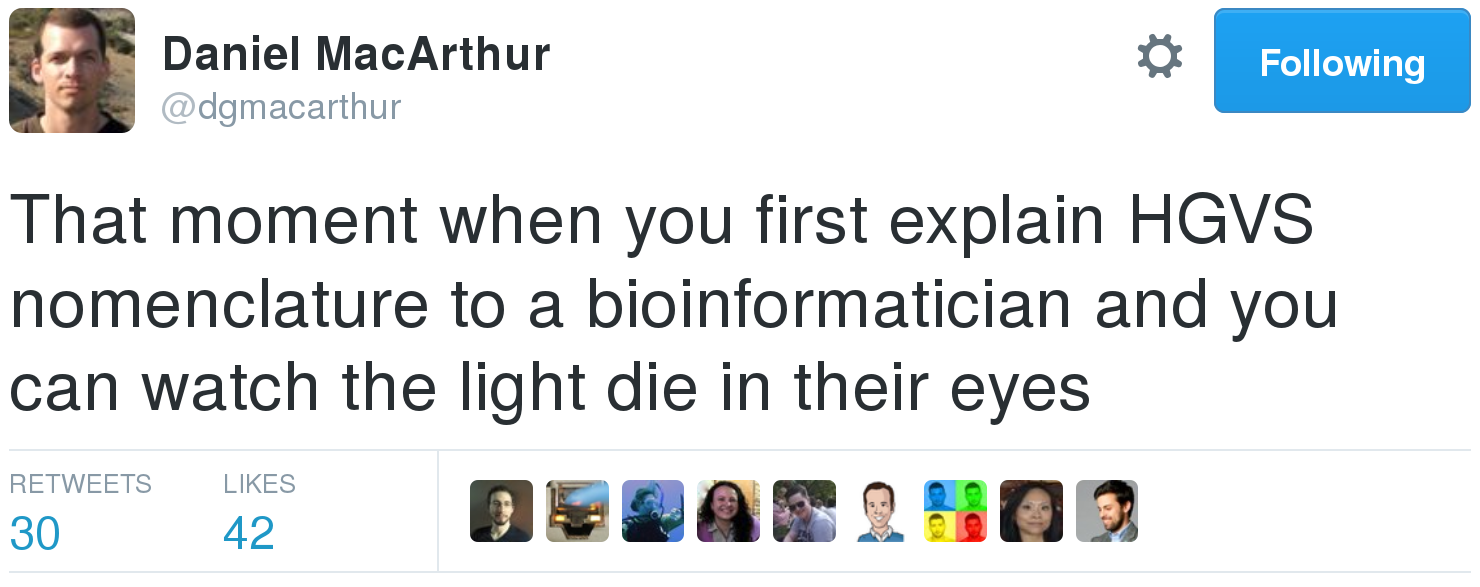
\includegraphics[width=0.7\textwidth]{pictures/twitter.png}
  \end{center}
  \pause
  \begin{block}{Popular opinion}
    \begin{itemize}
      \item Unfortunately, the above is just one of many similar expressions
      \item ``complex'' and ``confusing''
      \item Risc of alienating bioinformatics community
    \end{itemize}
  \end{block}
\end{frame}


\begin{frame}
  \frametitle{\textcolor{hgvs}{HGVS} nomenclature in tools}
  Tools:
  \begin{itemize}[<+->]
    \item \textbf{store}, \textbf{interpret}, \textbf{modify}, and
      \textbf{generate} variant descriptions
    \item are likely to hit corner cases
    \item are trusted to be correct\\[2em]
  \end{itemize}
  \uncover<4->{Tool developers need an unambiguous and complete
    specification.}
\end{frame}


\section{Proposal}


\frame{
  \frametitle{Specification of \textcolor{hgvs}{HGVS} nomenclature}

  \tableofcontents[currentsection]
}


\begin{frame}
  \frametitle{A more formal specification}

  \begin{block}{A set of unambiguous and exact rules}
    \begin{itemize}
      \item \textcolor{hgvs}{Correct} and \textcolor{hgvs}{complete}
      \item Should be \textcolor{hgvs}{leading}
      \item Does not have to be formal in the mathematical sense (yet)
    \end{itemize}
  \end{block}
  \pause
  Three parts:
  \begin{enumerate}
    \item Syntax
    \item Semantics
    \item Definition of prefered description
  \end{enumerate}
\end{frame}


\begin{frame}[fragile]
  \frametitle{1. Syntax \uncover<2>{\checkmark}}
  Describes the \textcolor{hgvs}{structure} of sentences in a language.\\[2em]

  Usually in the form of a \textcolor{hgvs}{grammar}: set of rules defining
  the syntactically valid sentences.\\[2em]

  \pause
  Published in 2011 (but not mentioned on \verb|hgvs.org/mutnomen|?).
\end{frame}


\begin{frame}
  \frametitle{Example of a grammar}

  \begin{center}
    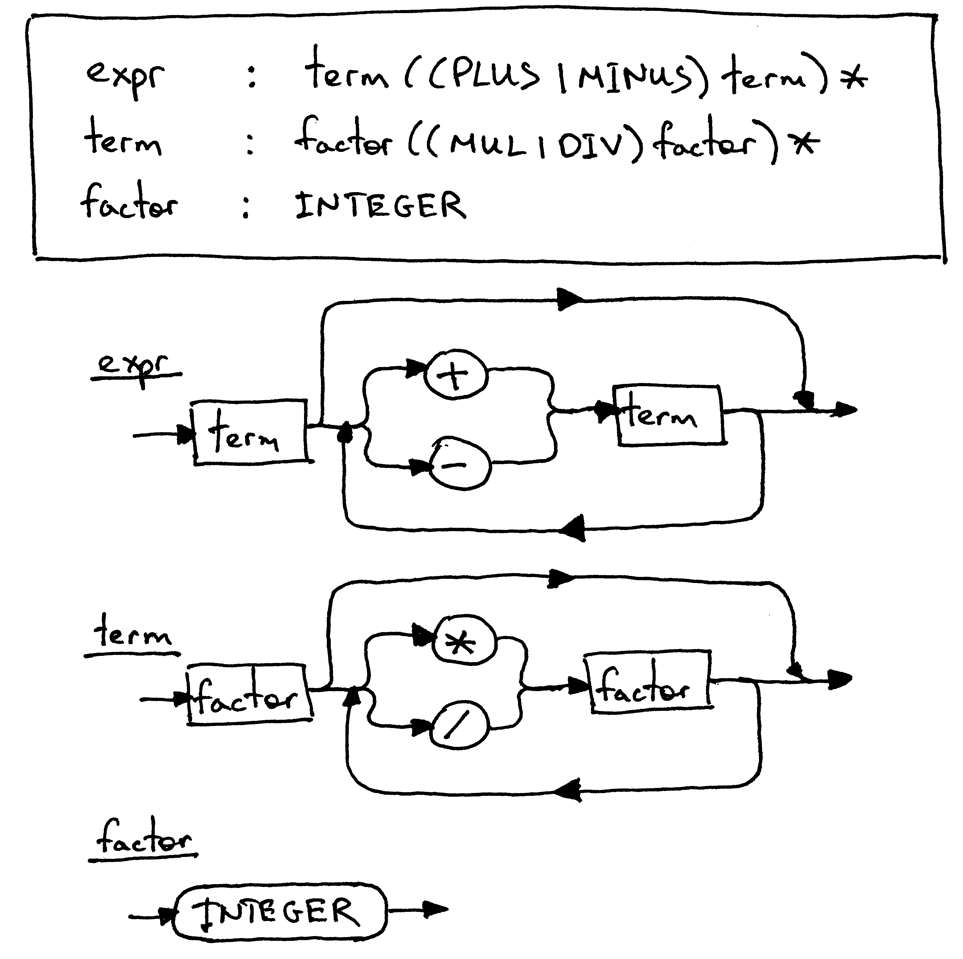
\includegraphics[width=0.75\textwidth]{pictures/grammar.png}
    % https://ruslanspivak.com/lsbasi-part5/
  \end{center}
\end{frame}


\begin{frame}
  \frametitle{2. Semantics}
  Assigns \textcolor{hgvs}{meaning} to (some) sentences in a language.\\[2em]

  Formal semantics are used in logic and the study of programming
  languages.\\[2em]

  Different approaches:
  \begin{itemize}
    \item Denotational semantics (complex)
    \item Operational semantics (similar to interpretation)
    \item Axiomatic semantics (based on logic)
  \end{itemize}
\end{frame}


\begin{frame}
  \frametitle{Example of an operational semantics}
  \begin{center}
    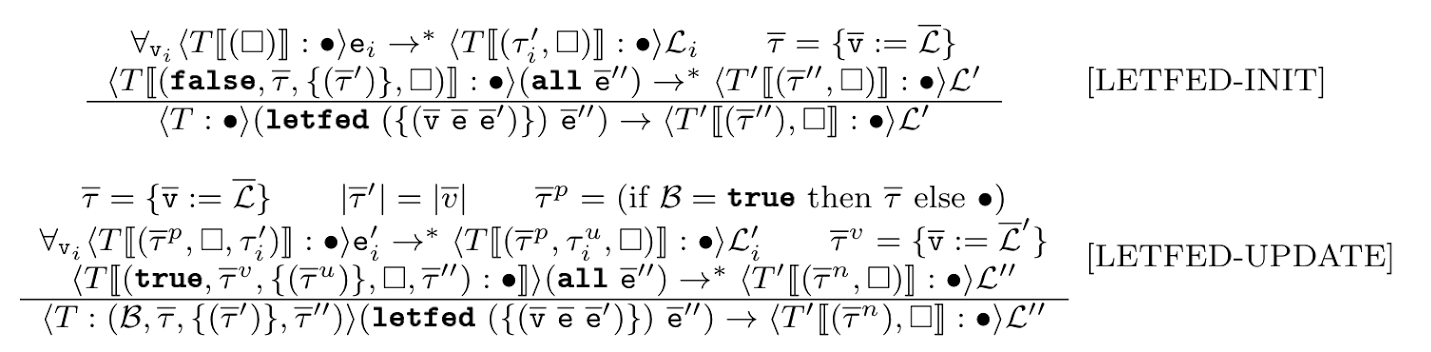
\includegraphics[width=1.1\textwidth]{pictures/semantics.png}
    % http://jakebeal.blogspot.nl/2013/01/operational-semantics-of-proto.html
  \end{center}

  \pause
  What\textinterrobang
\end{frame}


\begin{frame}
  \frametitle{A formal semantics for \textcolor{hgvs}{HGVS}?}

  True formal semantics are very mathematically heavy-weight, so we might aim
  a bit lower.\\[2em]

  Find a balance between mathematical rigor, feasibility, and practical
  applicability, without sacrificing correctness.\\[2em]

  \pause
  Best approach is an open question.
\end{frame}


\begin{frame}[fragile]
  \frametitle{3. Definition of prefered description}

  A variant can have more than one description:
  \begin{itemize}[<+->]
    \item \verb|NG_016465.4:g.12_15dup|
    \item \verb|NG_016465.4:g.13_16dup|
    \item \verb|NG_016465.4:g.15_16insTATC|
    \item \ldots\\[2em]
  \end{itemize}

  \uncover<4->{For a set of semantically equivalent descriptions, which one is
    the \textcolor{hgvs}{prefered} description?}
\end{frame}


\begin{frame}[fragile]
  \frametitle{Universe of variant descriptions}
  \begin{center}
    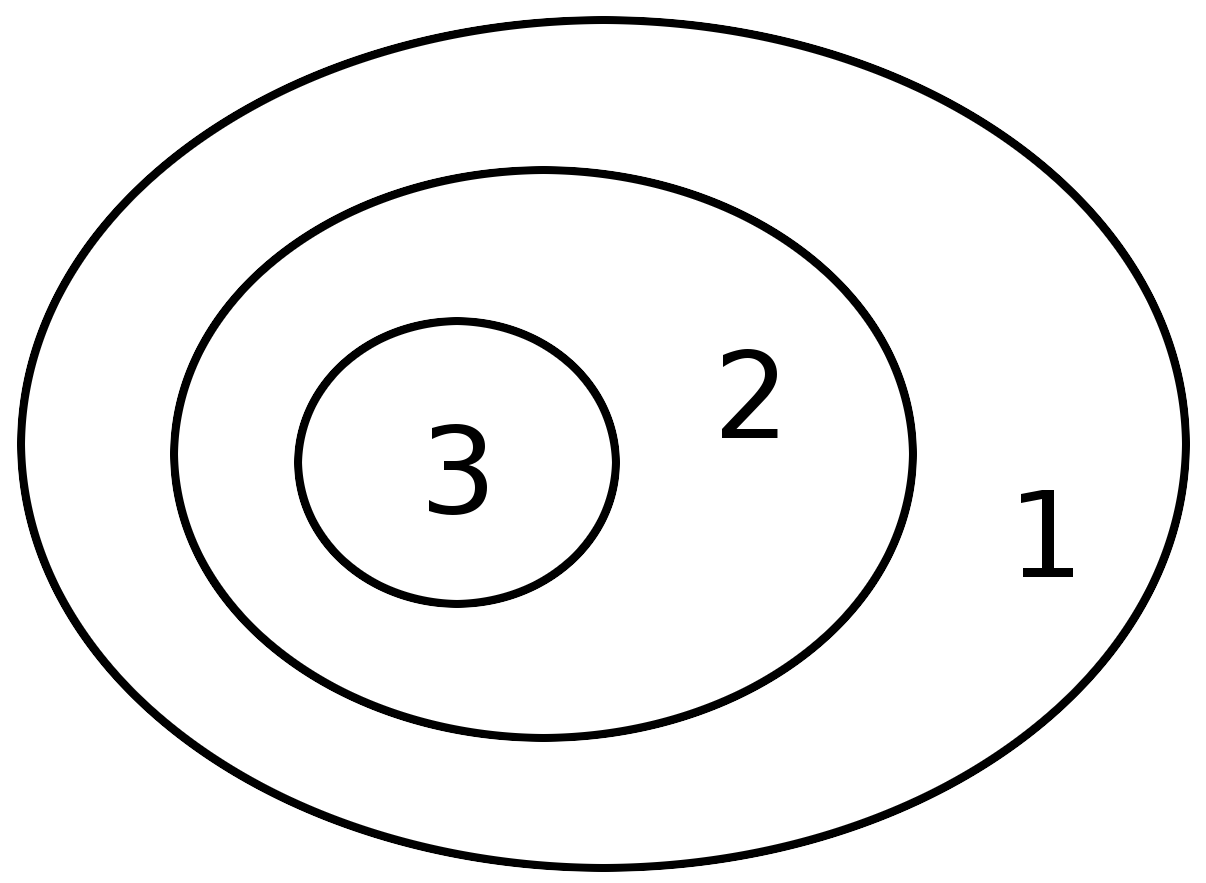
\includegraphics[width=0.7\textwidth]{pictures/descriptions.png}
  \end{center}
  \begin{enumerate}
    \item Syntactically valid descriptions
    \item Semantically valid descriptions
    \item Prefered descriptions
  \end{enumerate}
\end{frame}


\begin{frame}
  \frametitle{Prefered descriptions}

  Common practice is to prefer the \textcolor{hgvs}{shortest} description.\\[2em]

  This is a valid (though not completely unambiguous) definition, but not
  \textcolor{hgvs}{constructive}.\\[2em]

  A constructive definition could be an algorithm as implemented in the
  Description Extractor.
\end{frame}


\section*{Discussion}


\begin{frame}
  \frametitle{Acknowledgments}

  Jonathan K. Vis\\
  Peter E.M. Taschner\\
  Jeroen F.J. Laros\\
  Johan T. den Dunnen
\end{frame}


\end{document}
